%============================================================
\chapter{The~RdRand instruction}  \label{chap:rdrand-instruction}
\par{
First public information about RdRand came sometime during year 
2011~\cite{IntelRdRandFindAbout}, a~year before the~CPUs with it were released
 and~Intel itself sends patches to~add support into Linux in summer of~the~same 
 year~\cite{KernelRdRand}. Later, RdRand was added between Linux entropy 
 sources for {\tt /dev/[u]random}. According to~known 
 information~\cite{TheodoreTsoNSA}, Intel tried to~have {\tt /dev/[u]random} rely
  only on their instruction, but that was denied. 
}

\par{
After disclosure of~extends of~NSA spying activities by~Edward Snowden 
in summer of~2013~\cite{GuardianNSA,DailymailNSA}, a~petition for removing 
RdRand from Linux entropy sources was created~\cite{PetitionRdRand}. 
Although supported by~just 8 signatures, it got wide attention on 
information-technology aimed news pages and~magazines, like Slashdot.org~\cite{PetitionRdRandSlashdot}. The~petition was closed after Linus Torvalds 
responds with scorn:
}
\begin{quote} \par{\dots}
\par{
Short answer: we actually know what we are doing. You don't.
}
\par{
Long answer: we use rdrand as \_one\_ of~many inputs into the~random pool, 
and~we use it as a~way to~\_improve\_ that random pool. 
So even if rdrand were to~be back-doored by~the~NSA, our use of~rdrand 
actually improves the~quality of~the~random numbers you get 
from {\tt /dev/random}.
}
\par{\dots}
\end{quote}

\section{History}\label{sec:intel-history}
\par{
This is not for the~first time Intel is producing a~HW RNG. Around 1999, 
their chipsets of~8xx series had a~TRNG~\cite[chapter 1.3.5]{Intel810Manual}\cite{RNGTools} 
as part of~the~Intel FWH (82802AB or 82802AC) component.
This RNG was analog -- a~thermal noise was affecting a~resistor. 
The~noise was amplified and~forwarded to~a~voltage--controlled oscillator. 
Its output was combined with another oscillator with much higher frequency 
and~the~drift between these two frequencies provided the~requested entropy~\cite{IntelRNGAnalysis}.
}
\par{
Pairs of~generated bits were digitally processed, using Von Neumann Corrector to~enhance its statistical properties by~removing some bias. Due to~this, the~RNG has a~variable bitrate, averaging around 75 Kbit/sec.
}
\begin{table}[h!]
  \begin{center}
    \begin{tabular}{|c|c|}
      \hline
      Input Bits &  Output\\
      \hline  
      0, 0 & None\\
      0, 1 & 1\\
      1, 0 & 0\\
      1, 1 & None\\
      \hline
    \end{tabular}    \caption{A~Von Neumann corrector}
    \label{fig:VonNeumannCorrector}
  \end{center}
\end{table}

\newpage

% --------------------------------------------------------
\section{Intel Secure Key}\label{sec:intel-secure-key}
\par{
The~Intel Secure Key (ISK) uses cascade construction, combining a~HW RNG
 with CSPRNG into one sealed block on CPU, which is compliant with many 
 security standards, including NIST SP800-90, FIPS-140-2, and~ANSI 
X9.82~\cite{IntelDRNGGuide}. Although it is impossible to~audit it, there was found 
 no evidence of~low entropy or anything that would deny the~security standards 
 compliance - neither with tests in \fullref{sec:testing:stat-testing}, nor any other 
 tests anyone else did\footnote{I assume that such revelation would become 
 quickly known and~broadly discussed, but all tests I have found have 
 the~same conclusion as mine.}.
 }

% --------------------------------------------------------
\section{Physical Implementation}\label{sec:ISK-physical}
\par{
One important thing about ISK with a~big impact on the~performance, but also price 
of~that solution is that there is only one unit on a~die and~the~unit should be
 the~same on all CPUs\footnote{We didn't find the~"be the~same" officially confirmed and~it can change in future CPUs. But empirical test results made on range of~different CPU types provided the~same characteristics, with exception of~Intel Xeon CPUs as is described in the~\ref{chap:testing}.}~\cite[Chapter. 3.1]{IntelDRNGGuide}.
Because all processing units (PUs)\footnote{Two physical cores with 
hyper-threading count as four PUs.} on one die share the~RNG, one thread 
reading random numbers from it can never be faster than 
$Total speed  \frac{1}{PUs}$. The~effect of~this is that the~performance is
 scalable until amount of~PUs and~the~maximum output speed are exceeded 
 (see \fullref{sec:testing:performance-testing}), and~price of~the~CPU is less 
 affected.
}

\par{
Each ISK unit consists three basic parts: A~hardware entropy source, 
a~conditioner and~a~{\em deterministic random bit generator} (DRBG)
\cite{IntelDRNGGuide}. The~frequency of~the~RNG is independent 
on the~rest of~the~CPU and~is set to~800 MHz. 
}
\begin{figure}[h!]
  \centering
 \includegraphics[width = 10cm,keepaspectratio]{fig/ISK-scheme.pdf} % Or .pdf
%\includegraphics[width=10cm,keepaspectratio]{fig/ISK-scheme}
\caption{An Intel Secure Key unit}
\label{fig:ISK-unit}
\end{figure}


% ....................................................
\subsection{Entropy Source}
\par{
The~entropy source is a~metastable circuit, with unpredictable behavior based 
on thermal noise~\cite{UnderstandingRdRandElectronic}.
In figure~\ref{fig:ES-circuit}, the~middle (red) part is the~heart 
of~the~circuit, a~RS-NOR latch. As its {\em reset} and~{\em set} inputs 
are wired together, when an impulse is brought on these inputs, the~latch sets 
to~1 or 0 based on thermal noise. To~provide better distribution, there is 
the~bottom (blue) negative feedback. Based on the~output of~the~latch, charge 
on capacitors in the~negative feedback is adjusted and~then this negative 
feedback slightly shifts the~chance for next bit to~be opposite. The~longer 
is a~sequence of~the~same bits, the~higher charge is on the~capacitors 
and~bigger effect it has.
}

\par{
Finally, when the~latch is settled in one state, the~top (green) part 
of~the~circuit detect it, saves the~bit (and~send it further), wait 
a~little time and~then it sends a~pulse on the~R/S inputs of~the~latch 
to~produce a~new bit. This entropy source has its own frequency, different 
from the~rest of~the~RNG, about 3~GHz.
}
\begin{figure}[h!]
  \centering
 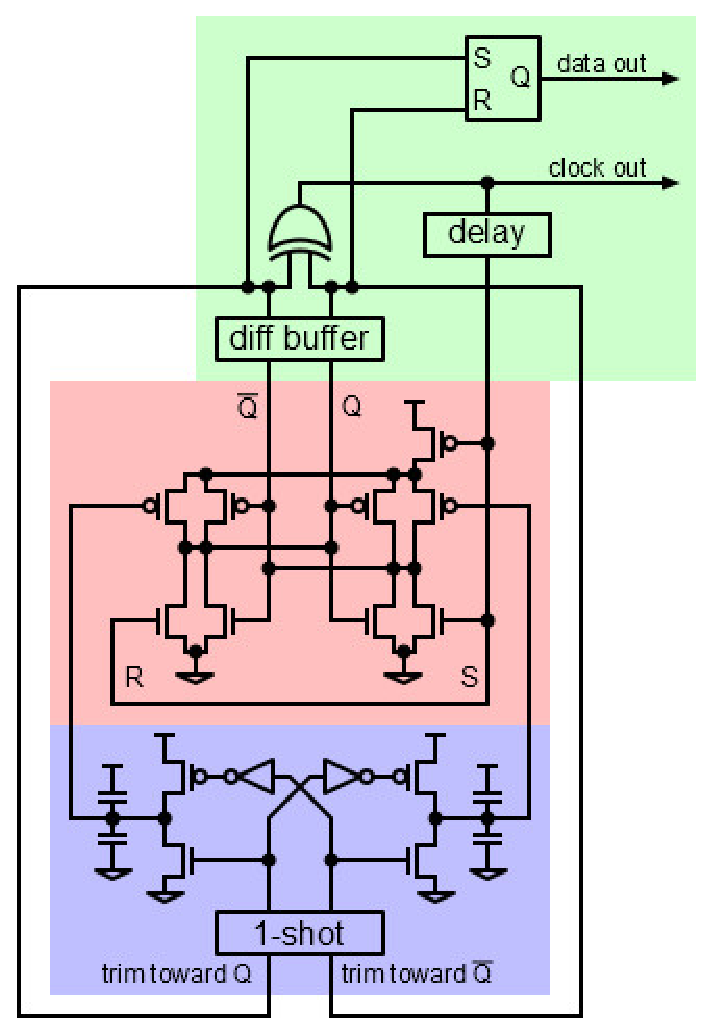
\includegraphics[width=6cm,keepaspectratio]{fig/entropy-source-circuit} % Or .pdf
%\includegraphics[width=10cm,keepaspectratio]{fig/ISK-scheme}
\caption{Circuit scheme of~the~entropy source~\cite{UnderstandingRdRandElectronic}. }
\label{fig:ES-circuit}
\end{figure}

% ....................................................
\subsection{Conditioner}
\par{
The~entropy source provides random bits with some entropy, 
but due to~implementation and the~feedback, it can be unbalanced 
and~produce values in something close to~oscillating patterns. 
For this reason, there is the~conditioner that adds them to~a~256 bit pool, 
make a~set of~XOR and~AES operations over lower and~upper half of~the~pool 
and~test health of~the~pool\footnote{The~health check is done by~counting six 
different bit patterns in the~256--bit pool and~comparing the~counts 
with empirically chosen values. The~pool is healthy only if the~numbers are 
in the~specified ranges.
}~\cite{AnalysisOfDRNG,UnderstandingRdRandElectronic}. 
If the~pool is not healthy, the~set of~operations is repeated. 
}
% ....................................................
\subsection{DRBG}\label{subsec:DRBG}
\par{
Because the~output speed of~the~conditioner is too slow (just 256 bits per few 
microseconds), 
a~deterministic random bit generator is connected to~the~256 bit pool 
and~every few microseconds (if the~pool is healthy) takes it as a~new seed. 
This pseudo random generator then computes 65.536 bits values using 
a~128-bit AES and~put them to an~output buffer. 
From there, they can be taken by~the~RdRand instruction after 64-bit 
blocks\footnote{64 bits are always taken out, no matter what size is 
the~target register of~the~instruction. Thus, it is not possible to~achieve the~full 
speed of~the~DRBG on 32-bit system, as there is no difference for the~Intel 
Secure Key usage from pulling 64 bits. Just some bits are thrown away. 
See \fullref{subsec:testing:differences} for a~performance test.}~\cite{AnalysisOfDRNG,UnderstandingRdRandElectronic}. 
Reseeding of~the~DRBG is required after all 1024 blocks are used, 
but usually it will reseed more frequently, 
about each 10 microseconds~\cite[Chapter~4.4]{IntelDRNGGuide}.
}
% ....................................................
\subsection{Built-in Self-Tests (BIST)}
\par{
Intel Secure Key contains also built-in self-tests. After a~reset, the~BIST at first test 
health of~the~DRBG and~conditioner, then it tests the~entropy source. In the~first 
part, ES is disconnected, a~previously determined bit sequence is 'generated' 
and~the~BIST checks the~output with a~built-in value. In second phase, 
the~entropy source is connected and~few sequences are generated. 
If the~entropy source would be bad, the~previously checked health check in conditioner would detect it. 
}

\par{
In case one of~the~BIST parts would not be finished correctly and~the~RdRand 
instruction is called, just zeros are returned and~carry flag is cleared~\cite{AnalysisOfDRNG}.
}

% --------------------------------------------------------
\section{Existing Usages} 
\par{
RdRand is already used in Linux kernel for both blocking and~non-blocking pools. For the~non-blocking pool({\tt /dev/urandom}), it is possible to~completely feed the~pool with RdRand~\cite{KernelRdRand}. For blocking pool ({\tt /dev/random}), the~RdRand is used as one of more entropy sources in {\tt drivers/char/random.c}.
}

\begin{lstlisting}[frame=none, basicstyle=\footnotesize\ttfamily, language=C, numbers=none, numberstyle=\tiny\color{black},caption= {Adding RdRand (and~any other platform-depending HW RNG) to~blocking pool with XOR, at line 1042 in {\tt drivers/char/random.c}~\cite{random.c}. }]
for (i = 0; i < LONGS(20); i++) {
	unsigned long v;
	if (!arch_get_random_long(&v))
		break;
	hash.l[i] ^= v;
}
\end{lstlisting}

\par{
Another well-known and~widely spread system already using RdRand is OpenSSL. This library added the~support in version 1.0.1~\cite[Chapter. 3.2 Generation]{OpenSSLRandomNumbers}. There the~RdRand is provided as one engine of~many and~requires to~be explicitly enabled.
}

\begin{lstlisting}[frame=none, basicstyle=\footnotesize\ttfamily, language=C, numbers=none, numberstyle=\tiny\color{black},caption= {Simplified example of~usage of~RdRand in OpenSSL~\cite{OpenSSLRandomNumbers}. }]
OPENSSL_cpuid_setup();
ENGINE_load_rdrand();
ENGINE* eng = ENGINE_by_id("rdrand");
ENGINE_init(eng);
ENGINE_set_default(eng, ENGINE_METHOD_RAND);

// Here use the engine with some RAND_ method

ENGINE_finish(eng);
ENGINE_free(eng);
ENGINE_cleanup();
\end{lstlisting}

\par{
In Windows~8, RdRand is used for example during boot for {\tt ASLR} {\em (Address Space Layout Randomization)}~\cite{WindowsASLR,WindowsHeap}.
}

% --------------------------------------------------------
\section{Security}\label{sec:security}
\par{
Security of~the~RNG is important, but it is hard to~check. During the~last few years,
 the~possibility of~hardware Trojans (malicious manipulation during 
 the~manufacturing process) gained attention, but none was yet found. This doesn't 
necessarily means that no such exists, because detection methods are 
much more difficult than with their software kindreds, and~frequently destructive. 
}

\par{
If such Trojan is not detected in software because of~altering verifiable outputs 
(like AES HW Acceleration, which would not encrypt the~data), 
there is not much other ways, than to~slice the~chip and~optically inspect it. 
The~verification against a~"golden chip" is expensive, destructive and~slow 
and~requires to~have the~"golden", trusted chip for comparison.
Yet it can find alterations in circuits that could open some backdoors. 
But recently, another possible attack vector was described by~international group
 of~scientists in their work {\em Stealthy Dopant-Level Hardware Trojans}~\cite{DopantAttack}, 
 in which they directly presented such attack on the~Intel's RdRand.
}

\par{
This~new category of~attack is not modifying the~circuits' layout 
and~is undetectable by~the~optical inspections, because it affects the~functionality
 of~transistors instead of~changing the~layout. By~slight changes 
 in doping\footnote{Doping means adding specific impurities to~the~clear silicon 
 to~change its electric properties.}, the~modified gate can become static.
}

\par{
While with a~correct RdRand an attacker has a~chance of~$ 1/2^{128}$ to~correctly guess 
a~random number, the~described attack could increase the~chance to~
$ 1/2^n$~\cite[Chap. 3.2, page 9]{DopantAttack}, but the~output of~such
 modified RdRand is still looking randomly. In the~work $n = 32$ is achieved,
while it still pass NIST random number test suite.
}

\par{
This kind of~attack (predictability) is different from what the~authors of~the~petition~\cite{PetitionRdRand} for removing RdRand from {\tt /dev/random} fears. Their point is that RdRand, as a~part of~the~CPU, can actively try to~reduce entropy of~the~pool. If the RdRand knows with which values its output is XORed (they can be in cache of~the~CPU), it can produce inverted value and~effectively impact the~entropy pool. But I don't have enough understanding of~this Linux subsystem to~be able to~evaluate this claim.
}
%============================================================
